
\tikzstyle{every picture}+=[remember picture]
\section{Projeto do Controlador a Eventos discretos}

\begin{frame}{Projeto do Controlador a Eventos discretos}
  \begin{enumerate}
   \item Projetar o controle\pause 
   \item Implementar o Controle \pause PLC - Ladder
\end{enumerate}
\end{frame}

\begin{frame}{Exemplo de Sistema}
\begin{figure}[H]
  \centering
  \includegraphics[width=0.8\textwidth]{cipnExample/schemePresentation.tikz}
  \caption{Exemplo de sistema a ser controlado.}
  \label{fig:cipnexamplescheme}
\end{figure}
% \note{
%   \begin{enumerate}
%    \item Projetar o controle\pause 
%    \item Implementar o Controle \pause PLC - Ladder \pause
%    \item Observar entradas e saídas\pause
%    \item Obter caminhos\pause
%    \item Identificar usando DAOCT 
%    \end{enumerate}
%  }
\end{frame}


\begin{frame}{Rede de Petri Interpretada para Controle}
\begin{figure}[H]
  \centering \includegraphics[width=\textwidth]{cipnExample/cipnPresentation.tikz}
  \caption{Exemplo de Rede de Petri interpretada para controle.}
  \label{fig:cipnexample}
\end{figure}
\end{frame}

\begin{frame}
  \begin{figure}[H]
    \centering
    \resizebox{0.7\textwidth}{!}{
   \includegraphics{cipnExample/cipnLadderPresentation.tikz}}
 \caption{Rede de Petri do exemplo implementada em Ladder.}
  \label{fig:cipnexampleLadder}
\end{figure}\note{método demonstrado por MOREIRA e BASILIO (2013)}
\end{frame}

\begin{frame}{Datalog}
  \note{
    Uma vez implementado o controle no PLC, é feita a observação. PLC Siemens possui
    os blocos functionais mostrados para gravar os dados num arquivo csv.\\
    Explicar cada bloco
  }
   \begin{figure}[ht]
       \begin{minipage}[b]{0.3\linewidth}
         \centering
 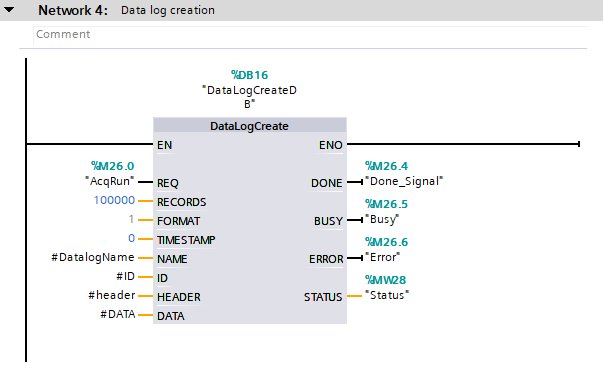
\includegraphics[width=\textwidth,clip,trim={0 0.8cm 3cm 0}]{tutorial/create}
       \end{minipage}
       \begin{minipage}[b]{0.3\linewidth}
         \centering
 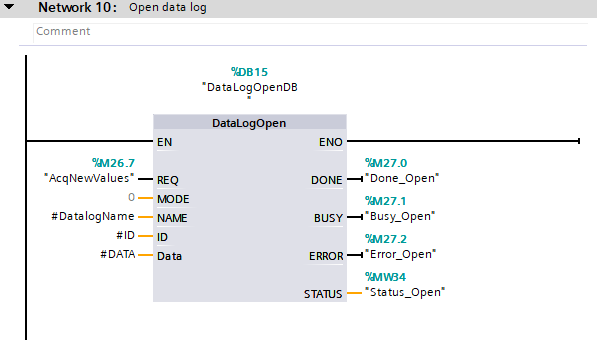
\includegraphics[width=\textwidth,clip,trim={0 0.4cm 3cm 0}]{tutorial/open}
\end{minipage}
       \begin{minipage}[b]{0.3\linewidth}
         \centering
	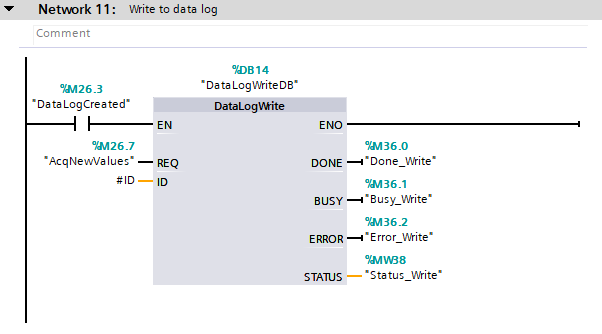
\includegraphics[width=\textwidth,clip,trim={0 0 3cm 0}]{tutorial/write}
       \end{minipage}
       \hspace{0.5cm}
       \begin{minipage}[b]{0.3\linewidth}
           \centering
	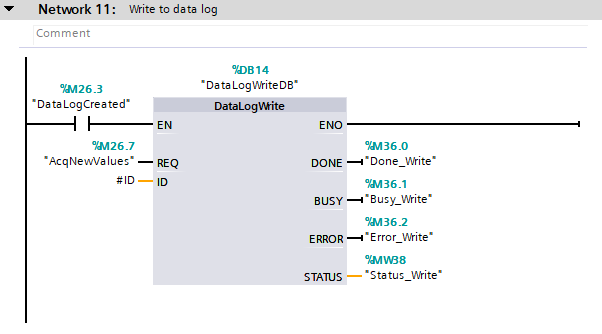
\includegraphics[width=\textwidth,clip,trim={0 1cm 3cm 0}]{tutorial/write}
       \end{minipage}
       \begin{minipage}[b]{0.3\linewidth}
           \centering
           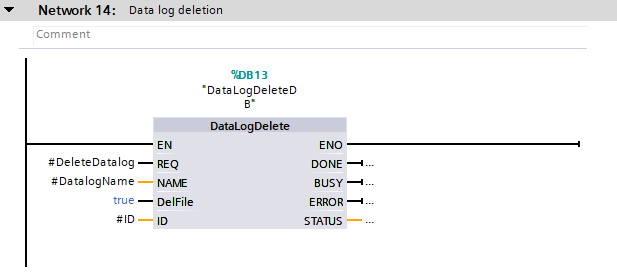
\includegraphics[width=\textwidth,clip,trim={0 -0.8cm 3cm 0}]{tutorial/delete}
       \end{minipage}
  \caption{Blocos Funcionais para gravação de dados.}
   \end{figure}
\end{frame}


\begin{frame} \begin{figure}
    \centering
\begin{tikzpicture}[scale=0.8]
     \def\corner{0.15in};
     \def\cornerradius{0.02in};
     \def\lwidth{0.02in};
     \def\h{1.1in};
     \def\w{0.85in};
     \def\nline{10};
     \def\iconmargin{0.1in};
     \def\topmargin{0.3in};
     \foreach[count=\i] \filename in {file.csv}
     {
     \coordinate (nw) at ($(-0.05in*\i,-0.15in*\i)$);
     \coordinate (ne0) at ($(nw) + (\w, 0)$);
     \coordinate (ne1) at ($(ne0) - (\corner, 0)$);
     \coordinate (ne2) at ($(ne0) - (0, \corner)$);
     \coordinate (se) at ($(ne0) + (0, -\h)$); 
     \filldraw [-, line width = \lwidth, fill=white] (nw) -- (ne1) -- (ne2)
      [rounded corners=\cornerradius]--(se) -- (nw|-se) -- cycle;
     \draw [-, line width = \lwidth] (ne1) [rounded corners=\cornerradius]-- (ne1|-ne2) -- (ne2);
     \node [anchor=north west] at (nw) {\scriptsize \tt \filename};
     \foreach \k in {1,...,\nline}
     {
       \draw [-, line width = \lwidth, line cap=round] 
         ($(nw|-se) + (\iconmargin,\iconmargin) + (0,{(\k-1)/(\nline-1)*(\h - \iconmargin - \topmargin)})$)
           -- ++ ($(\w,0) - 2*(\iconmargin,0)$);
     }
   }
   \node[inner sep=0pt] at (8,0) {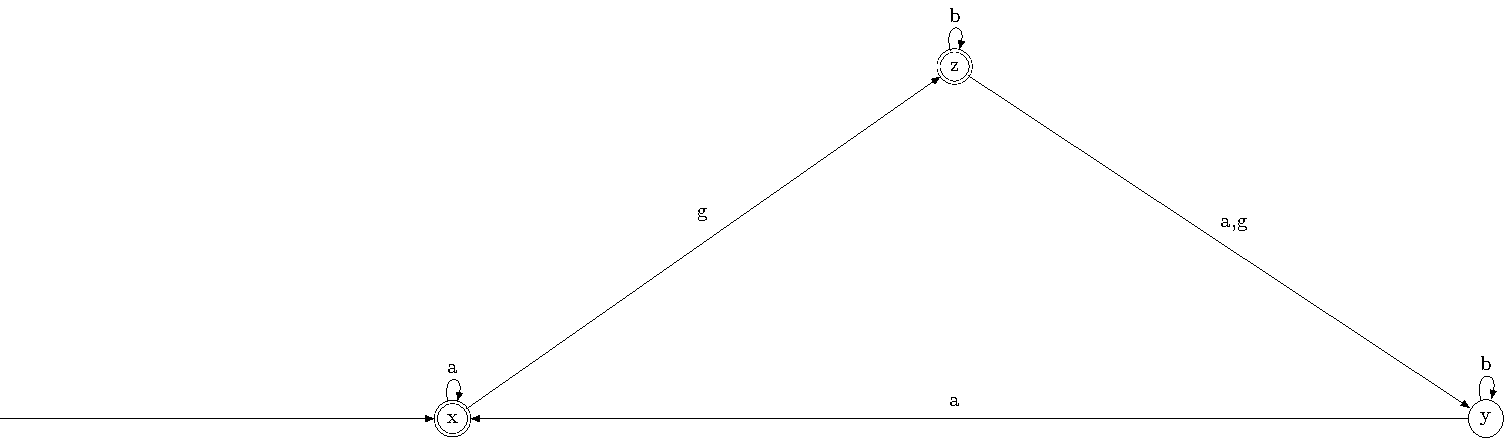
\includegraphics[width=0.4\textwidth]{example/example.pdf}};
   \draw[->] (1,0) to [bend left] (6,1);
   \draw (4,1.7) node {daoct};
   \end{tikzpicture}
  % \includetikzfigure[width=\textwidth]{example/stdin}
  \caption{Modelo identificado a partir do arquivo csv.}
  % \label{fig:identExamplekone}
\end{figure}
\note{
progama daoct criado para fazer obtenção dos caminhos da forma mostrada no
capítulo anterior, modificar os caminhos usando a formula descrita e
implementar o algoritmo de modelagemdo DAOCT.
}
\end{frame}

%%% Local Variables:
%%% mode: latex
%%% TeX-master: "../presentation"
%%% End: